\todo{Brief paragraph summarizing what are we going to study
Description of the experimental platform HW OS Compilers,
OpenBLAS
} 

\begin{figure*}[]
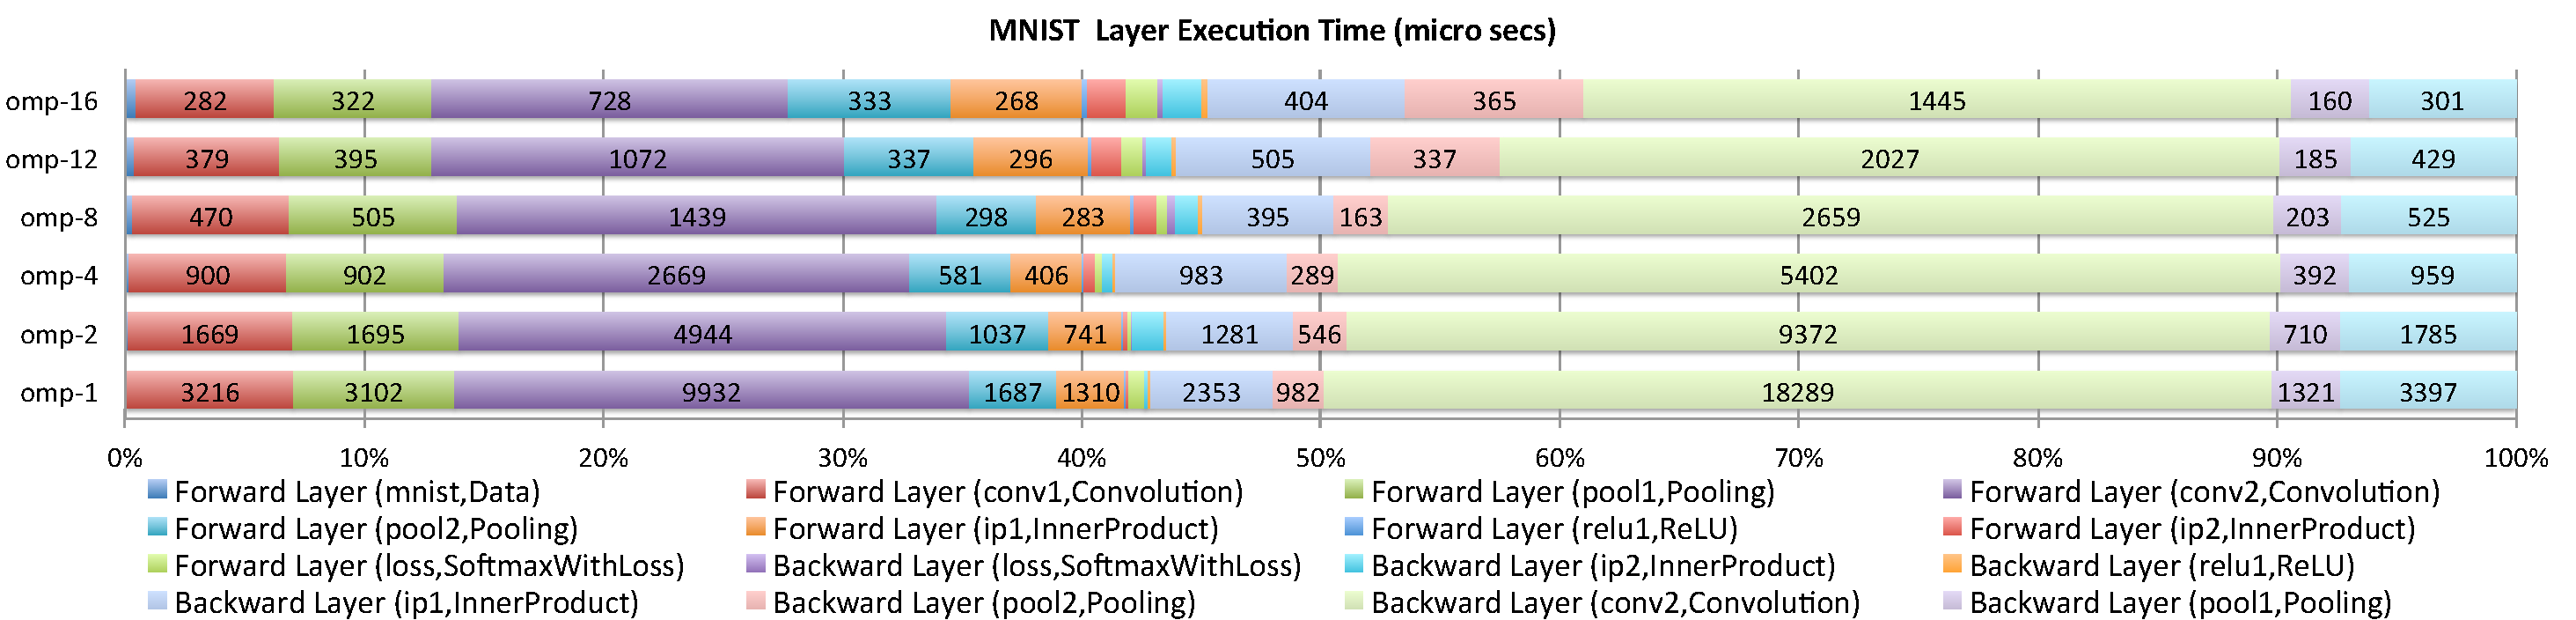
\includegraphics[width=\linewidth]{figures/mnist-rel-abs-time.pdf}
\caption{\todo{MNIST - Relative and absolute execution layer time.}}
\end{figure*}

\begin{figure*}[]
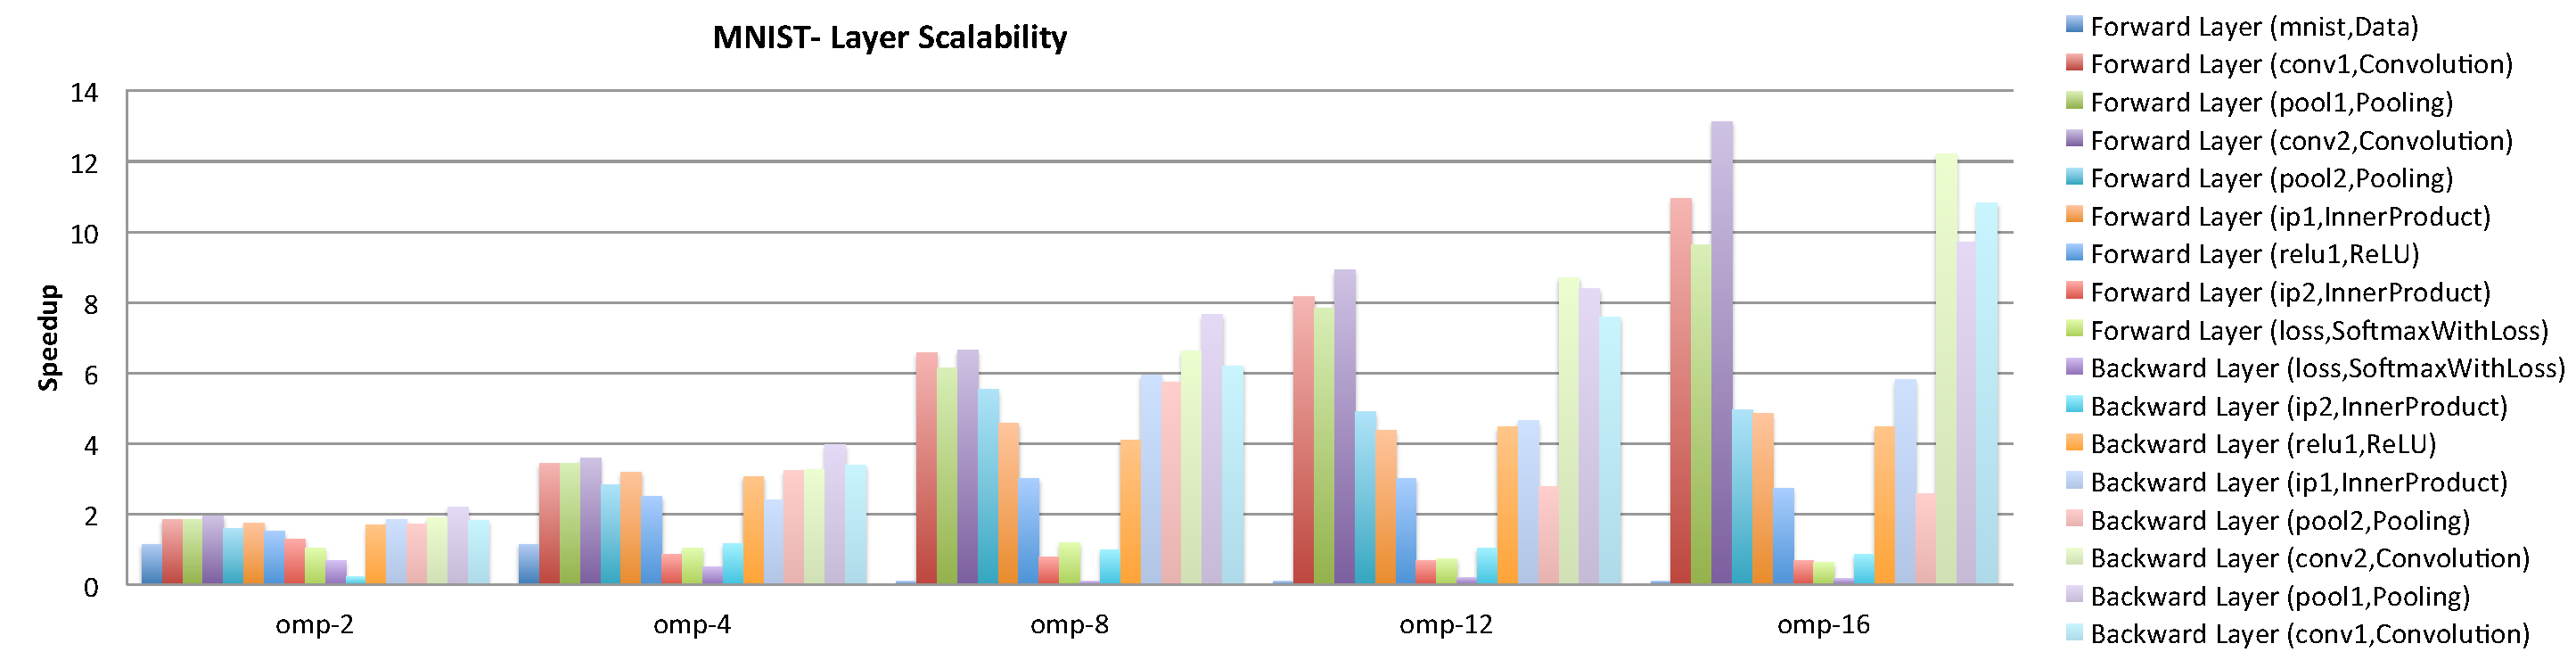
\includegraphics[width=\textwidth]{figures/mnist-scalability-layer.pdf}
\caption{MNIST - Layer Scalability}
\end{figure*}

\subsection{MNIST dataset}
For the performance analysis of the MNIST dataset we have first 
developped a per-layer study bothg coarse-grain and fine-grain parallelizations.For the coarse-grain case we identify what are the main limiting 
peformance factors. Then we describe the overall performance of the 
coarse-grain parallelization. 

\subsubsection{Coarse-grain Layer Performance}
Figure \ref{fig-mnist-abs-rel} shows the absolute execution time per layer 
and the relative weight in the overall execution time. Horizontal bars 
correspond to executions with 1, 2, 4, 8, 12 and 16 threads. In general, 
two layers dominate the whole execution: the convolutional and pooling 
layers. No matter the number of threads, these two type of layers always 
account for almost 80\% of total execution time, adding their forward 
and backward phases. Notice that there are different instances of the 
same type of layer but with very different absolute execution time. 
For instance, the \emph{conv1} and conv2 layers, and in a smaller magnitude 
the pool1 and pool2 layers. After the convolutional and pooling layers, 
the next significant layer is the inner product ip1. The rest of layers, 
expose a very small contribution to the overall execution time 
(e.g.: loss, relu and ip2 layers in their forward and backward phases).
In general, notice that in each horizontal bar there is a zone where the 
work in each layer phase decreases. This corresponds to the center part, 
composed of the forward and backward phases of pool2, ip1, relu, ip2 and loss.
This behaviour is associated to the dimensionality reduction that neural 
networks do, and affects the work granularity for the parallelization process.
Moreover, this behaviour limits the overall scalability of the training process.

Figure \ref{fig-mnist-scalability} shows the scalability curve of each layer. 
We identify three layer behaviours. First, notice the u-shape of the 
scalability trends for any number of threads. The center points 
correspond to the layers that we have previously identified as not 
significant in the overall execution time (e.g.: loss, relu and ip2 layers). 
These layers do not scale at all, but they do not represent a limitation for 
the overall performance. The two sides on the center values correspond 
to the forward and backward phases of the rest layers. For these, we detect 
two types of layer behaviour. 

Layers ip1 and pool2 present very poor scalability curves. 
For ip1, in both the forward and backward phases, the layer 
presents speedups of 4,58 and 5,93 for the forward and backward 
phases respectively and with 8 threads. The layer does not improve 
the speedup with more threads. The pool2 layer exposes the same 
behaviour with maximum speedup of 5.52 and 5.73 with 8 threads in 
the forward and backward phases respectively. The reason for this 
behavior is two fold. First, notice the two layers are immediately 
stacked one on top of the other. This means that the 
output of the pool2 layer is the input for the ip1 layer. It happens 
that the blob shapes between the two layers do not match. The pool2 
layer is parallelized according to its input blob dimensions, and 
produces its output blob (input blob for ip1) following the resulting 
work and data distribution coming out from the parallelization. When 
it comes the execution of the ip1 layer, its parallelization is done 
according to its input blob dimensions (output blob of pool2), which do 
not match those of the input blob for the pool2 layer. Thus, theres is 
an unvoidable lost of locality for the execution of the ip1 layer. 
Second, both layers suffer from a poor granularity when executing with 
more thatn 8 threads. In Figure \ref{fig-mnist-abs-rel} we observe that 
with more than 8 threads the forward and backward phases of the two layers 
are in the range of 350 microseconds.

Layers conv1, pool1 and conv2 present good scalability curves. They 
correspond to the layers in both sides of the center part of the 
scalability layer curves. In general, these layers respond well to the 
increments on the number of threads. This is explained by two factors. 
First, all these layers expose a considerable amount of work, as it has 
been indicated with Figure \ref{fig-mnist-abs-rel}. Second, all of them 
are stacked one next to each other within the network, and all of them 
match their input/output blob dimensions. Thus, data locality is 
preserved along the their execution in both the forward and backward phases.
We have detected that although being exactly the same layer, the conv1 
and conv2 layers have close to a 10\% difference in speedup. 
In particular, the conv2 layer exposes greater speedups than conv1. 
This happens more noticeably with more than 8 threads and for the 
forward phase. The difference between the two layers is the position 
they occupy in the layer stack. Conv1 is the immediate layer after the 
data layer in the MNIST network. The data layer is responsible for
feeding the network with data samples. The layer executes sequentially, 
so the data associated to all images generates a memory footprint that is 
not matching the one generated along the parallel execution of the 
conv1 layer. Therefore, the conv1 layer suffers from a poor data 
locality with its immediate previous layer.

\begin{figure}[]
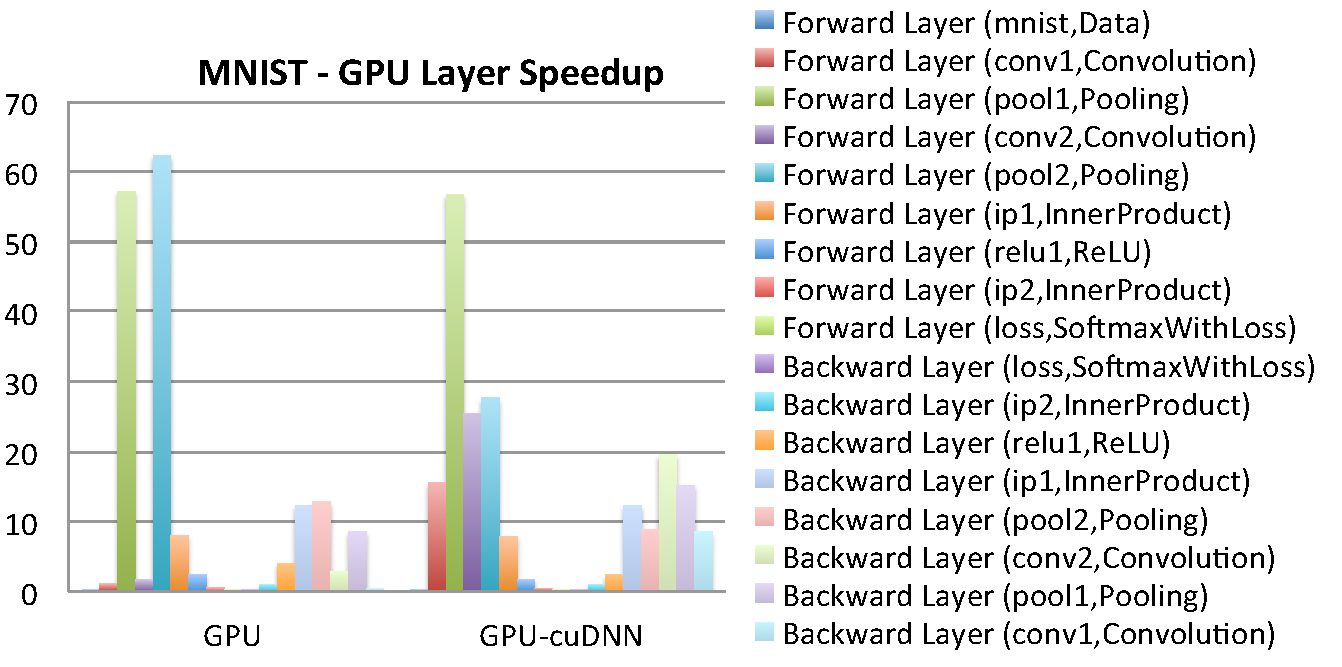
\includegraphics[width=\linewidth]{figures/mnist-gpu-layer-speedup.pdf}
\caption{\todo{CAPTION}}
\end{figure}

\subsubsection{Fine-grain Layer Performance}
\todo{- In 2012, Caffe won the ILSVRC2012-winning SuperVision
model and caching IO.
- CPU version is not comparable in terms of the optimization
efforts.
- cuDNN is not general enough, it is totally oriented to image
classification NO GENERALITY. Main success for accelera-
tion of convolutions reaching speedups of XXXX.
Make an example: no current support for LSTM in cuDNN,
other examples ??
Build the case for cuDNN NOT being a general framework for
DNN.
Compare with GPU BLAS level approach (and GPU-cuDNN?)
}

\begin{figure}[b]
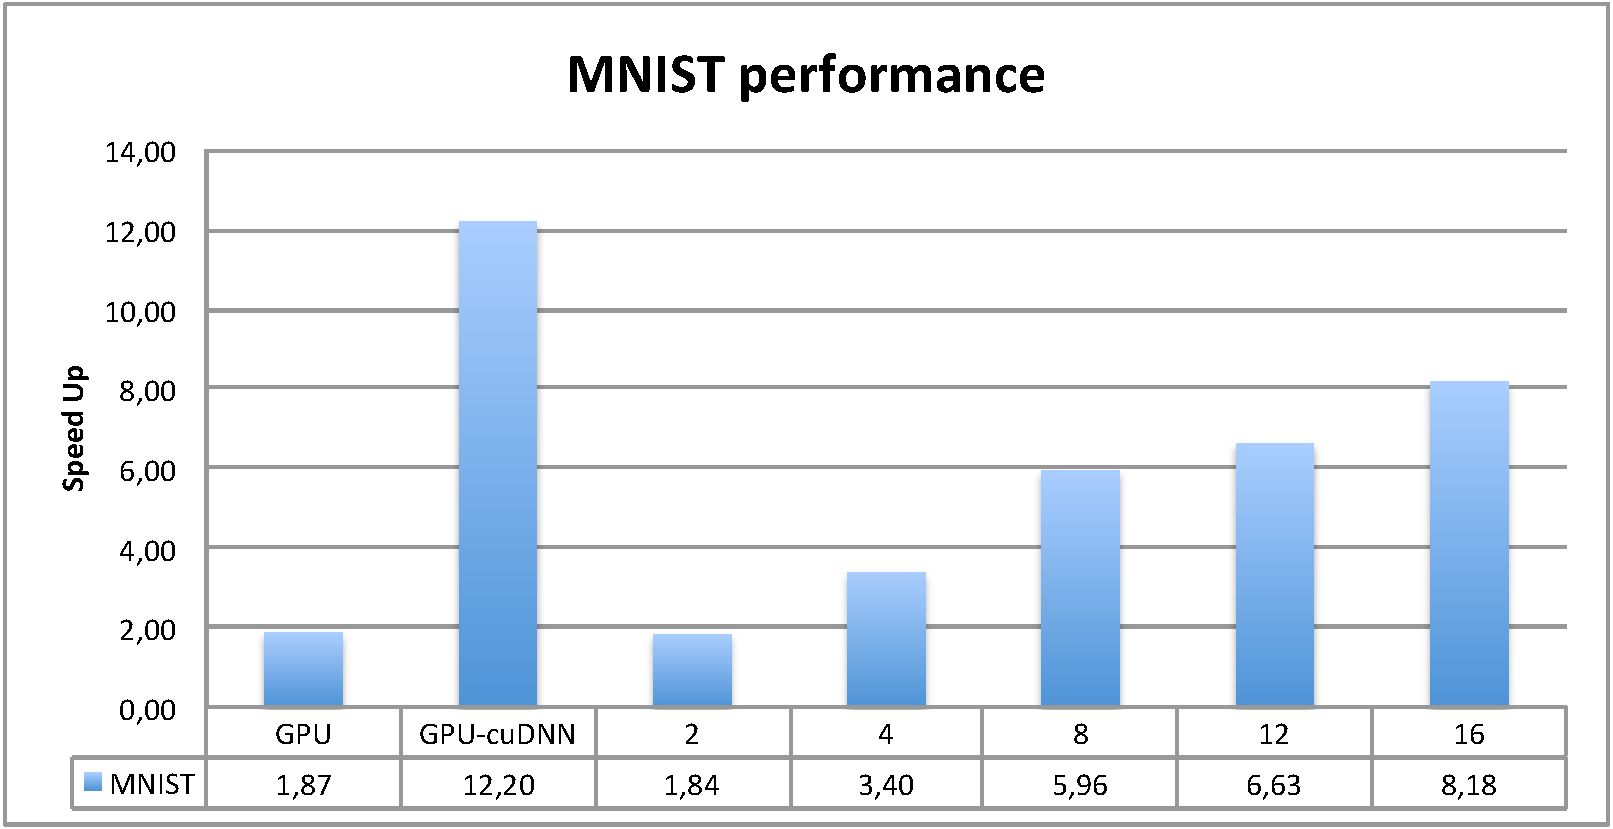
\includegraphics[width=\linewidth]{figures/mnist-abs-perf-all.pdf}
\caption{\todo{CAPTION}}
\end{figure}

\subsubsection{Overall Performance}
Figure \ref{fig-mnist-overall} shows the overall performance of
the coarse-grain parallelization and the fine-grain parallelization in 
its two verions GPU and GPU-cuDNN. The coarse-grain reaches a speedup 
close to a 6x with 8 threads, and 8x with 16 threads. The lack of 
the scalability for the CPU version is related to the poor scalability 
of fine-grained layers that when executing with 16 threads drag down 
the performance. In addition, we suspect the serial initialization of 
the network structures is giving a suboptimal memory allocation in 
the NUMA nodes. All of this is affecting the final scalability of 
the coarse-grain version. The fine-grain GPU version shows a 
modest speed up close to 2x. The reason for this difference is related 
to the performance of the convolutional layers. In general, this version 
corresponds to a base line defined by the Caffe native implementation 
of the GPU acceleration. It represents a case for the performance the DNN 
community can obtain with a fine-grain parallelization and very significant 
coding efforts. Remember that within Caffe, all layers have to have 
their corresponding GPU implementation. In conclusion, the coarse-grain 
approach minimizes the coding efforts and delivers better performance 
levels. Of course, when compared to the cuDNN case, the fine-grain 
approach makes the difference. It delivers a 12x speedup. But solutions 
like the cuDNN framework are only available when the layer types and 
their implementation have become a product and are no longer in a 
research stage. Thus, they can have a highly optimized implementation. 
For a DNN framework aimed to give support for 
research in new network architectures with novel layer types, 
the fine-grain parallelism imposes hard recoding efforts. In contrast, 
the coarse-grain option is much more immediate and has been proved to be 
more effective.



\subsection{The CIFAR-10 case}

The dataset is divided into five training batches and one test batch, each with 10000 images. The test batch contains exactly 1000 randomly-selected images from each class. The training batches contain the remaining images in random order, but some training batches may contain more images from one class than another. Between them, the training batches contain exactly 5000 images from each class. 
\subsubsection{Coarse-grain Layer Performance}
\todo{Similar as MNIST}

\subsubsection{Fine-grain Layer Performance}
\todo{Similar as MNIST}

\subsubsection{Overall Performance}
\todo{Similar as MNIST}

\subsection{Coarse-grain Performance Limiting Factors}
We have identified several factors that affect the batch-level
parallelization of the Caffe DNN framework. These factors are
layer dependant and are mainly related to specificities of the
layers that determine their work distribution, memory footprint,
data privatization and ordered operations. The following subsec-
tions describe these limiting factors.

\textbf{Sequential memory allocation}: the network memory allocation
happens during the network initialization. This process is sequen-
tial, which causes the layer memory be allocated following a
pattern generated by the initialization code. In terms of perfor-
mance, this pattern is not compatible with those that arise during
the training process.

\textbf{Locality between layers:} the input/output relation across layers
defines a lost of data locality for specific layers. During the for-
ward and backward phases, each layer distributes the work ac-
cording to the dimensions of the input blobs. Regarding the data
locality, it is possible that input and output blobs do not match
their dimensions. Consequently, the work distribution and thread-
data association defined in one layer will not match that one of the
next immediate layer in the stack, causing some data movement
across the memory hierarchy.

One particular case of this situation corresponds to the data
layers in Caffe. These layers feed the network with input data
organized in batches. Data layers execute in single-thread mode.
Therefore, a one thread first accesses all data and then the data is
distributed across the cores and the memory hierarchy when the
first parallel processing layer in the network is executes in paral-
lel. 

\textbf{Work unbalance:} coarse grain parallelism is open to work unbal-
ance. For the Caffe case, we have detected that batch-level paral-
lelism defines very heavy iterations for the parallelized loops.
Therefore, one single loop iteration can cause a high unbalance
between the executing threads. In general, threads receive the
same number of iterations (e.g.: under a static scheduling). But it
is possible that some of the threads receive one more iteration
than other threads when the number of samples in the batch is not

\textbf{Work granularity:} as previously described, neural networks try
to perform a dimensionality reduction over the processed data.
And this affects the size of the working sets in the network layers.
At some level in the network, the input/output blobs start decreasing their sizes. When this happens, a thread level parallelization
starts suffering from too small work granularity with poor performance levels.

\textbf{Data privatization and reduction operations:} specifically in the
backward phase, the network coefficients are updated per each
sample in the batch. At batch-level, this requires mutual exclusion
mechanisms to guarantee a correct update. Data privatization has
been needed for this purpose. Caffe is implemented following an
object-oriented design and object privatization (e.g.: blobs) has
performance implications regarding the invocation of object constructor/destructor.


